
%%%%%%%%%%%%%%%%%%%%%%% file typeinst.tex %%%%%%%%%%%%%%%%%%%%%%%%%
%
% This is the LaTeX source for the instructions to authors using
% the LaTeX document class 'llncs.cls' for contributions to
% the Lecture Notes in Computer Sciences series.
% http://www.springer.com/lncs       Springer Heidelberg 2006/05/04
%
% It may be used as a template for your own input - copy it
% to a new file with a new name and use it as the basis
% for your article.
%
% NB: the document class 'llncs' has its own and detailed documentation, see
% ftp://ftp.springer.de/data/pubftp/pub/tex/latex/llncs/latex2e/llncsdoc.pdf
%
%%%%%%%%%%%%%%%%%%%%%%%%%%%%%%%%%%%%%%%%%%%%%%%%%%%%%%%%%%%%%%%%%%%


\documentclass[runningheads,a4paper]{llncs}

\usepackage{amssymb}
\usepackage{amsmath}
\setcounter{tocdepth}{3}
\usepackage{graphicx}

\usepackage{url}
\urldef{\mailsa}\path|{daniel.opitz, sebastian.graf, nikolai.baudis}@student.kit.edu|
\newcommand{\keywords}[1]{\par\addvspace\baselineskip
\noindent\keywordname\enspace\ignorespaces#1}

\begin{document}

\mainmatter  % start of an individual contribution

% first the title is needed
\title{Bioinformatics Practical Documentation}

% a short form should be given in case it is too long for the running head
\titlerunning{Bioinformatics Practical Documentation}

% the name(s) of the author(s) follow(s) next
%
% NB: Chinese authors should write their first names(s) in front of
% their surnames. This ensures that the names appear correctly in
% the running heads and the author index.
%
\author{Sebastian Graf\and Nikolai Baudis\and Daniel Opitz}
%
\authorrunning{Bioinformatics Practical Documentation}
% (feature abused for this document to repeat the title also on left hand pages)

% the affiliations are given next; don't give your e-mail address
% unless you accept that it will be published
\institute{Karlsruhe Institute of Technology, Institute of Theoretical Informatics,\\
Kaiserstrasse. 12, 76131 Karlsruhe, Germany\\
\mailsa\\
\url{http://www.informatik.kit.edu/}}

%
% NB: a more complex sample for affiliations and the mapping to the
% corresponding authors can be found in the file "llncs.dem"
% (search for the string "\mainmatter" where a contribution starts).
% "llncs.dem" accompanies the document class "llncs.cls".
%

\toctitle{Lecture Notes in Computer Science}
\tocauthor{Authors' Instructions}
\maketitle


\begin{abstract}
In this documentation we describe our implementation of algorithmic DNA sequence alignment building on the TKF91 maximum likelihood evolutionary model. The goal of this project was to implement an application that computes the pairwise sequence alignment using the aforementioned model and that is highly optimized for performance. In order to maximize the performance, we utilized vectorization using SSE3 and AVX vector intrinsics. Further, we implemented optimizations such as an efficient memory layout, memoization, and address alignment, which all together keep overheads to a minimum. In addition, we ensured that our optimized program prevents numerical underflow.

%\keywords{Keywords}
\end{abstract}


\section{Introduction}
\label{sec:introduction}

In \cite{TKF91}, Thorne, Kishino, and Felsenstein presented a method for aligning DNA sequences using a maximum likelihood approach under the assumption of an explicit statistical model of evolution including insertion, deletion and substitution as basic operations on the DNA sequences. The evolutionary model assigns a weight to each basic operation for the dynamic programming procedure to compute the resulting alignment using maximum likelihood. 

For the substitution model we assume the Felsenstein standard phylogenetic nucleotide substitution model. The algorithm computes the optimal score for the sequence alignment in three matrices, which ultimately leads to the following dynamic programming rules: 
\[
\begin{aligned}
  M^0(i,j)&=\frac{\lambda}{\mu}\pi_{a_i}\overline{p_0}(t)max\{M^0(i-1, j), M^1(i-1,j), M^2(i-1,j)\}\\
  M^1(i,j)&=\frac{\lambda}{\mu}\pi_{a_i}max\{P_{a_i \rightarrow b_j}(t) p_1(t), \pi_{b_j}\overline{p_1}(t)\}\\
          &\quad\quad max\{M^0(i-1, j-1), M^1(i-1,j-1), M^2(i-1,j-1)\}\\
  M^2(i,j)&=\pi_{b_j}\lambda\beta(t)max\{M^1(i,j-1), M^2(i,j-1)\}
\end{aligned}
\]
Where $\lambda$ and $\mu$ denote the birth and death rate, $\pi_x, x \in \{A,C,G,T\}$ denotes the equilibrium probability of the nucleotides, $P_{x \rightarrow y}$ the transition probability from $x$ to $y$, and $\overline{p_n}(t)$ the probability that after time $t$ a mortal link has exactly $n$ descendants. The values for $t$, $\lambda$, $\mu$, and $\pi$ are predetermined by the evolutionary model. The values for $\overline{p_n}$ can be precomputed in constant time.


\section{Implementation}
\label{sec:implementation}

In this section, we explain the details of our implementation.  Before we describe our vectorization approach, the prerequisites are explained: Section~\ref{ssec:dynprogramming} describes the dynamic program and the arising wavefront parallelism we exploited in our implementation. In section~\ref{ssec:memorylayout}, we depict our choice for an efficient memory layout, which is required to take full advantage of the vectorization. Continuing with Section~\ref{ssec:memo}, we describe how to we could cache most intermediate computations, before we explain our choice for a vectorization approach in Section~\ref{ssec:vectorization}. In addition to that, Section~\ref{ssec:dataalignment} outlines our considerations regarding the alignment of the data, marking an important part of the vectorized implementation. Finally, in Section~\ref{sec:evaluation} we describe the test and benchmark suites that we used to take decisions regarding the memory layout and vectorization approaches and the resulting performance measurements.


\subsection{Dynamic Programming and Wavefront Parallelism}
\label{ssec:dynprogramming}

Our main goal in this project was to speed up the computation of the alignment for two sequences of DNA. The alignment should be computed following the maximum likelihood approach that has previously been described in Section~\ref{sec:introduction}. \textit{Dynamic Programming (DP)} is a well explored technique to solve a certain class of otherwise computation intensive problems (exhibiting \textit{overlapping subproblems} and \textit{optimal substructure}) such as said sequence alignment in an efficient way. Another great benefactor to use dynamic programming is the fact that it allows to parallelize the computation along the anti-diagonals of the dynamic programming matrix in a very efficient and easy way. This parallelization of a DP algorithm along the anti-diagonals is referred to as wavefront parallelism. The key principle of this concept is that matrix entries of the same anti-diagonal $d$ can be computed independently from each other if all the matrix entries of the preceding anti-diagonal $d-1$ are known. In this way, the computation of an anti-diagonal can be seen as a vector operation and therefore it presents a promising approach to make efficient use of vector intrinsics.


\subsection{Memory Layout}
\label{ssec:memorylayout}

As a preliminary we will briefly introduce the memory layout of the DP matrices. Since it is crucial for the computation that the algorithm operates with high data locality to take advantage of the CPU cache, we permuted the indexing scheme of the DP matrix in a way that matrix entries that are neighbors on a matrix anti-diagonal are also neighbors in memory. Figure~\ref{fig:indexing} shows how the matrix is internally represented in memory. The matrix is layed out neither column- or row-major in memory, but linearly along its anti-diagonals. 

\begin{figure}[ht!]
  \centering
  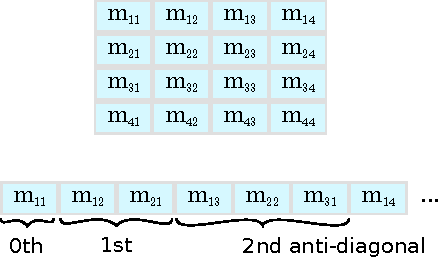
\includegraphics[scale=0.9]{figures/indexing.pdf}
  \caption{Memory layout for the dynamic programming matrix}
  \label{fig:indexing}
\end{figure}

This indexing is achieved using a modified version of the \textit{Cantor pairing function}, where a tuple is assigned to an offset. Originally, the Cantor paring function $\pi$ assigns an integer to a pair of integers as in $\pi: (\mathbb{N}, \mathbb{N}) \rightarrow \mathbb{N}$. Since the size of the DP-matrix is defined by the length of the sequences (and is not infinite), the pairing function needs to be modified so that it takes a tuple of two integral numbers from the interval $[0..\textrm{length}(\textrm{Sequence 1\textbar2})]$. Therefore, the matrix is divided into three parts: the \emph{opening}, \emph{middle}, and \emph{closing part}. In the opening part, the modified paring function is equal to the original function; in the middle and closing part, the modified pairing function is calculated by subtracting an offset from the original pairing function. This offset is again calculated using the original Cantor pairing function.

\begin{figure}[ht!]
  \centering
  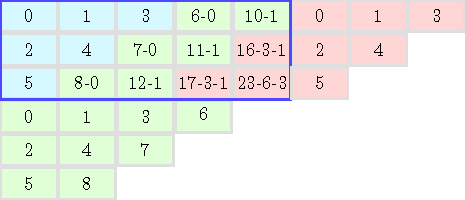
\includegraphics[scale=0.9]{figures/pairingfunc.pdf}
  \caption{Indexing scheme for the anti-diagonals}
  \label{fig:pairingfunc}
\end{figure}

In Figure~\ref{fig:pairingfunc}, the calculation of the indices for the anti-diagonals in a $5\times3$-matrix is visualized. The blue border shows the bounds of the DP matrix, the blue cells represent the opening part, the green cells inside the matrix the middle and the red cells inside the matrix the closing part. Green and red cells outside of the matrix boundaries show the Cantor pairing functions for the offset calculation for the middle and closing part, respectively. For this, only the first rows of those pairing functions are needed. 

Having established the indexing along the anti-diagonals for a single matrix,
the memory layout of the three DP matrices $M_0$, $M_1$, and $M_2$ has to be
defined.  The calculation of new values inside the DP algorithm requires values
from each of the three matrices.  Therefore, the access pattern inside the
matrices follows the same anti-diagonals.  In order to improve cache locality
while enabling efficient load and store operations, the matrix data has to be
arranged using a reasonable layout.  Based on these requirements, we evaluated
three matrix layouts, which are shown in Figure~\ref{fig:datalayout}:

\begin{figure}[ht!]
  \centering
  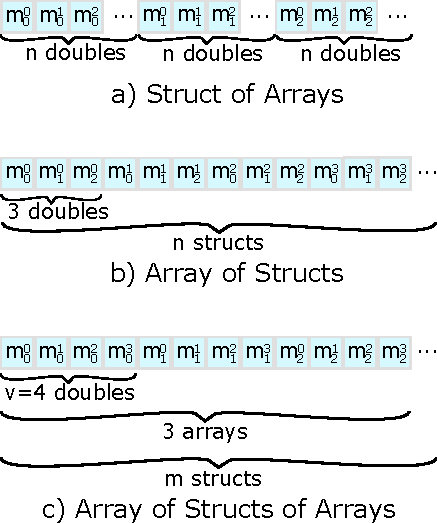
\includegraphics[scale=0.7]{figures/datalayout.pdf}
  \caption{Different data layouts for saving the anti-diagonals}
  \label{fig:datalayout}
\end{figure}

  \paragraph*{Struct of Arrays (SoA)} ({\small\texttt{struct \{ double m0[n], m1[n], m2[n]; \} data;}}) This layout entails the simplest load and store
operations. However, the three matrices are located in separate regions of
memory, which considerably impairs cache locality.

\paragraph*{Array of Structs (AoS)} ({\small\texttt{struct \{ double m0, m1, m2; \}
data[n];}}) This layout offers better cache locality by grouping values
closely together that are -- in most cases -- used at the same time. On the
other hand, loading and storing vectors requires deinterleaving and interleaving
them, which leads to several shuffle operations. 

\begin{figure}[ht!]
  \centering
  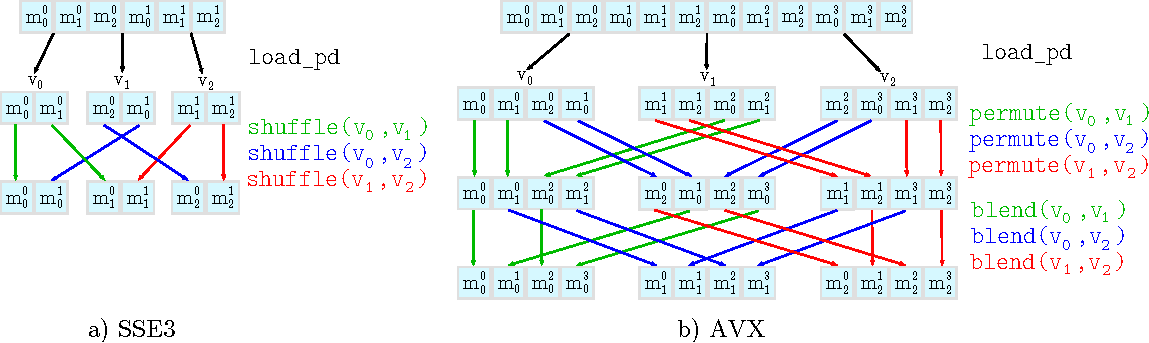
\includegraphics[scale=0.6]{figures/shuffle.pdf}
  \caption{Deinterleave operations for a) SSE3 and b) AVX vectors.}
  \label{fig:shufflesse}
\end{figure}

Figure~\ref{fig:shufflesse} illustrates those shuffle operations. For $m_x^y$, the subscript $x$ indicates
the index of the matrix and the superscript $y$ describes the element index of the SSE3/AVX vector.
The first row shows the data layout for the AoS strategy. Then an (aligned) \texttt{load} is 
performed to load the raw data into temporary vectors. After that the temporary vectors are 
permuted so that a single vector contains only elements from one of the tree DP matrices in
the correct order of the diagonal. Both SSE3 and AVX need to perform three \texttt{load} operations and 
three \texttt{shuffle}/\texttt{permute} operations. For AVX, we need to additionally perform three \texttt{blend} operations to
retrieve the data in correct order. 

\paragraph*{Array of Structs of Arrays (AoSoA)} ({\small\texttt{struct \{ double m0[v],
m1[v], m2[v]; \} data[m];}}) While this layout solves both of the previous problems,
grouping vectors in advance complicates calculations that use values from the
cells above:  These values would not lie within vector boundaries and would then
again require \texttt{shuffle}/\texttt{permute} operations or partial loads.

\paragraph*{} All three layouts have different performance characteristics
regarding cache locality and complexity of load and store operations.
After implementing prototypes for all three approaches to analyze their
performance, we decided to implement the AoS approach.  Interestingly, the complexity
of the \texttt{shuffle} operations outweighed the improved cache locality in the AoS and
AoSoA layouts, as seen later in Table~\ref{tbl:benchmark}. 


\subsection{Memoization}
\label{ssec:memo}

The model in \cite{TKF91} is highly parametric and it initially seemed inevitable to do non-trivial computations each step in the tight loop of the dynamic program. However, after analyzing which expressions could be precomputed and reused (i.e. memoized), we managed to reduce all computations to either an indirection, a summation, or a maximization operation.

Among the obvious savings were the expressions only dependent on the time parameter $t$, the birth rate $\lambda$ and the death rate $\mu$, all of which remain constant for the entire computation. Extrapolating on that observation, we realized that the steps in the DP algorithm share only a constant number of common subproblems: Once the nucleotides at the current indices in the sequences were available, the score could be computed solely in terms of the current nucleotide pair and the neighboring values in the dynamic programming matrix.

The memoization scheme for the possible transition penalties is shown in Figure~\ref{fig:memo}. The penalties $C^i$ take one or two nucleotides as parameters, rendering them amenable to memoization in a table of $4$ or $16$ entries, respectively. With just a total of $24$ memoized values, we could severely simplify the update steps expressed by $M^i$, which yielded a speedup of orders of magnitudes. Besides that, the simplification made possible a number of other important steps such as using log scores to prevent numerical underflow, since computing logarithms each step in the original formulation would have been too expensive. It also kept the translation to SIMD-enabled code manageable and the result leaves little room for conflicting design decisions in terms of performance.

At a later point, it became evident that the indexed loads from memoized penalty matrices caused quite a hit in performance. Spinning forth the idea of memoization, we precomputed a table of vector-sized elements, which we indexed by the specific permutation of the nucleotides. Building on an example utilizing AVX intrinsics, we would calculate a bijective map from a pack of four nucleotides to an integer denoting one of its $4^4 = 256$ different permutations (e.g. a perfect hash) for $C^0$ and $C^2$, and $4^{2 \cdot 4} = 65536$ for $C^1$ respectively. The map was effectively realized by a base conversion from the nucleotide quartet string to an unsigned integer by a sequence of bitwise operations.

Besides the fact that this approach would scale exponentially bad in space to wider vector registers, a constant $65536 \cdot 32$ bytes $= 2$ MB for $C^1$ in the case of AVX were tractable. Evaluating the resulting performance unfortunately revealed that too much time was spent populating the table for the practical inputs of our benchmark data. Since the table is purely dependent on the likelihood model (independent of the input sequences), it is however subject to reevaluation, should we extract the initialization of the likelihood model out of the DP initialization. The scaling to wider vector registers could be retained by loading a register in packs of four values.

\begin{figure}
\[
\begin{aligned}
  C^0(a)&=\frac{\lambda}{\mu}\pi_{a}\overline{p_0}(t)\\
  C^1(a, b)&=\frac{\lambda}{\mu}\pi_{a}max\{P_{a \rightarrow b}(t) p_1(t), \pi_{b}\overline{p_1}(t)\}\\
  C^2(b)&=\pi_{b}\lambda\beta(t)\\
  M^0(i,j)&=C^0(a_i)max\{M^0(i-1, j), M^1(i-1,j), M^2(i-1,j)\}\\
  M^1(i,j)&=C^1(a_i,b_j)max\{M^0(i-1, j-1), M^1(i-1,j-1), M^2(i-1,j-1)\}\\
  M^2(i,j)&=C^2(b_j)max\{M^1(i,j-1), M^2(i,j-1)\}
\end{aligned}
\]
\caption{Reformulation of the dynamic program step exposing the memoized sub-problems $C^i$}
\label{fig:memo}
\end{figure}


\subsection{Vectorization}
\label{ssec:vectorization}

We implemented a vectorized version of the computation of $M_0$, $M_1$, and
$M_2$ matrix entries, comprising \texttt{add}, \texttt{max}, \texttt{load}, and \texttt{store}
operations for both SSE3 and AVX.  Using these operations, $n$ elements of the
matrices are processed in parallel.  Depending on the location of the
anti-diagonal part that is processed, there are $0 < n \leq V$ elements in a vector
(with vector size $V = 4$ for AVX and $V = 2$ for SSE3). 

Although we ensured aligned access to a majority of the data (as will be explained in
Section~\ref{ssec:dataalignment}), the \texttt{load} and \texttt{store}
operations were implemented using \texttt{loadu\_pd} and \texttt{storeu\_pd}
SSE3 and AVX intrinsics. This does not represent a disadvantage for the
performance, since we could not identify significant performance impacts of
using unaligned intrinsics on aligned data.

To prevent our \texttt{store} operations from overwriting data at the edge
region of the matrices, we ensured that for vectors with size $n < V$ (i.e.,
not completely filled vectors) only $n$ elements are written back into the
matrices.  For the SSE3 version, this can be achieved by only writing the lower
part of the vector if its size is $1$.  For AVX, however, we covered all cases
where $n < V$ holds using a \texttt{maskstore\_pd} intrinsic and a store mask
for each possible value of $n$ (which basically only includes $3$, $2$, and $1$)
such that only the $n$ values we computed are written back into the matrices.

\subsection{Data Alignment}
\label{ssec:dataalignment}

When implementing the vectorization along the anti-diagonals, addressing the memory in the dynamic programming matrices as row-, or column-major matrices practically prevents any usage of efficient vector operations for loading the values from the matrices into vector registers. In such an implementation, the tight loop of the algorithm becomes heavily IO-bound. Therefore, the optimizations for the memory layout mentioned above have been made, so that \texttt{load} and \texttt{store} operations for copying data into vector registers could be utilized. Those vector \texttt{load} and \texttt{store} operations, however, come in two different flavors: There are \texttt{load} and \texttt{store} operations for aligned data and unaligned data. The latter can have a negative impact on the performance in comparison to the aligned loads (although, as mentioned in Section~\ref{ssec:vectorization}, loading aligned data using \texttt{loadu\_pd} holds no such penalty). But using aligned loads introduces yet another difficulty in storing the DP matrices: When loading the data from the matrices into SSE3 vector registers, the data has to be aligned on a $16$ byte boundary (respectively on a $32$ byte boundary for AVX).

\begin{figure}[ht!]
  \centering
  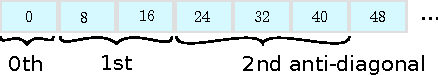
\includegraphics[scale=0.9]{figures/unaligned.pdf}
  \caption{Shift of the byte offset of the anti-diagonals}
  \label{fig:unaligned}
\end{figure}

Figure~\ref{fig:unaligned} shows how the byte offset for the anti-diagonals is shifted from one diagonal to the next. In order to easily find the aligned addresses for loading the vectors we made yet another change to the indexing function for the anti-diagonals. The main idea is to let each anti-diagonal start at a special aligned address. When iterating over anti-diagonal elements in a vectorized fashion, the vectors are then automatically constructed from data that is aligned to the required address offset.

The starting address for the diagonal is not the required alignment address for loading and storing the vectors, but a larger address minus the size of one double floating point value. This is due to the fact that the 0th row of the matrix is precomputed during the matrix initialization and therefore a value is never written to this row. Another reason for this decision is that it is impossible to load all vectors needed for the computation inside the tight loop of the algorithm from an aligned addresses.

\begin{figure}[ht!]
  \centering
  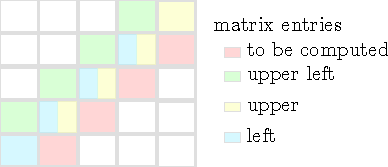
\includegraphics[scale=1.1]{figures/alignment.pdf}
  \caption{Outline of the data required for an operation in the DP loop}
  \label{fig:alignment}
\end{figure}

In Figure~\ref{fig:alignment}, the required values for the computation in the DP loop are shown (in this case for AVX, where the vector length is $4$ doubles). The matrix elements marked in red are the elements that are unknown and shall be computed in this step. For the computation of a single element three more elements from the two previous columns are needed. The element directly above (yellow) and left (blue) to the unknown element and the element located in diagonally upper left (green) need to be loaded from the DP matrices. The figure illustrates that (neglecting the asymptotically irrelevant corner cases) either one of these four conditions hold true:
\begin{enumerate}
  \item red and blue start on an aligned address, yellow and green do not
  \item red and yellow start on an aligned address, blue and green do not
  \item yellow and green start on an aligned address, red and blue do not
  \item red and green start on an aligned address, yellow and blue do not
\end{enumerate}

For the computation we need to perform three \texttt{load} operations in total for the blue, yellow, and green elements and one \texttt{store} operation for the red elements. Since the unaligned \texttt{store} operation holds a greater relative impact on performance in respect to the unaligned load operations, we ensured that either the first or the second condition is met. The first condition is ensured for the opening and middle part, the second condition is ensured for the closing part of the DP matrices.

We achieved the alignment of each anti-diagonal through a padding, which is inserted after each anti-diagonal. We realized this padding by modifying the indexing function into the matrices. In the final version of this indexing function for an anti-diagonal, a certain amount of array elements in the matrix buffer is skipped. Elements are skipped until the second element of the anti-diagonal is aligned with the vector intrinsics requirements. This way, some memory is wasted because it is not used, however it is asymptotically insignificant compared to the overall space complexity of the algorithm ($O(\textrm{length}(\textrm{Sequence 1}) \cdot \textrm{length}(\textrm{Sequence 2}))$).


\section{Evaluation and Testing}
\label{sec:evaluation}

\subsection{Benchmarks and Test Suites}
\label{ssec:benchmark}

An automated test suite is extremely valuable for refactoring and optimizing the code, in that it provides the confidence of being able to detect regressions early and get helpful hints on how to fix them. We used the \textit{ctest} module of \textit{CMake} to invoke a Python script driving our console wrapper through a number of inputs. As we also used a continuous integration service running the tests on new commits, we could easily spot when a change accidentally broke the build. This development process lead to a high level of satisfaction and faith to try out different ideas in separate branches, while immediately getting feedback.

When the most obvious optimizations were done and we began to make use of vectorization instructions, we realized a benchmark suite based on the alignment data sets from the University of Oldenburg\footnote{http://goo.gl/nlD4nb} using the Celero C++ benchmarking library\footnote{https://github.com/DigitalInBlue/Celero} to have a reliable way of validating performance of our different approaches.

From each of the six data sets, we picked ten nucleotide strings and computed all 45 pairwise alignments. We found that the median of five \textit{samples}, each of which consisting of the average of ten such \textit{iterations} (i.e. $5*10*45 = 2250$ alignments per data set) gave reliable performance estimates. As stated in Section~\ref{ssec:dataalignment}, we performed various performance comparisons based on this benchmark suite, such as the viability of different vector load and store schemes or the SoA, AoS, and AoSoA issue, of which the benchmark results on the reference hardware are depicted in Table~\ref{tbl:benchmark}. As already noted in Section~\ref{ssec:dataalignment}, we deemed the SoA approach the most performant.

\begin{table}[]
\centering
\label{tbl:benchmark}
\begin{tabular}{llll}
\begin{tabular}[c]{@{}l@{}}ms per iteration\\ (compared to best)\end{tabular} & SoA                & AoS                & AoSoA        \\
BDNF                                                                                      & 8.30 (1.01)        & {\bf 8.22 (1.00)}  & 8.51 (1.04)  \\
cytb                                                                                      & {\bf 26.19 (1.00)} & 29.07 (1.11)       & 29.65 (1.13) \\
RAG1                                                                                      & 20.88 (1.02)       & {\bf 20.56 (1.00)} & 20.94 (1.02) \\
RAG2                                                                                      & {\bf 24.64 (1.00)} & 25.09 (1.02)       & 25.83 (1.05) \\
RBP3                                                                                      & {\bf 35.26 (1.00)} & 36.35 (1.03)       & 37.62 (1.07) \\
vWF                                                                                       & 44.54 (1.01)       & {\bf 44.10 (1.00)} & 46.27 (1.05)
\end{tabular}
\caption{Benchmark results for SoA, AoS and AoSoA (from left to right)}
\end{table}


\section{Conclusion}
In this documentation we presented our implementation of the TKF91 evolutionary model for aligning sequences of DNA. Therefore we outlined the definition of an efficient memory layout, as well as measures to factor out complex computations during the tight loop in the DP algorithm. We presented our approach to the vectorization of the algorithm using SSE3 and AVX vector intrinsics and discussed how data can be efficiently aligned. Finally, the performance of the resulting application was tested and evaluated. 

As a final note, we would like to remark that keeping the data spatially coherent by adjusting the memory layout through interleaving the matrices did not result in the performance gain that had first been anticipated. Unfortunately, the penalty of the shuffling and blending during loading and storing vectors, which has been introduced by those memory layouts, almost perfectly outweighed the gain in cache locality, which can be seen in Table~\ref{tbl:benchmark} in Section~\ref{sec:evaluation}.

\bibliographystyle{plain}
\bibliography{mlalign}

\end{document}
